\documentclass[lang=cn,10pt]{elegantbook}

\title{自动控制原理:经典和现代}


\author{江布力·加尔肯别克}
\date{2022年9月}
\version{考研版0.0}
%\bioinfo{自定义}{信息}

\extrainfo{费曼学习法告诉我们:教是学的最高阶段}

\setcounter{tocdepth}{3}

\cover{control.jpg}

% 本文档命令
\usepackage{array}
\usepackage{color}
\newcommand{\ccr}[1]{\makecell{{\color{#1}\rule{1cm}{1cm}}}}

% 修改标题页的橙色带
% \definecolor{customcolor}{RGB}{32,178,170}
% \colorlet{coverlinecolor}{customcolor}

\begin{document}

\maketitle
\frontmatter

\tableofcontents

\mainmatter


\chapter{概述和数学基础}

\begin{introduction}
  \item 控制系统组成~
  \item 控制系统分类~
  \item 数学基础~
\end{introduction}

本章基本上就是对控制系统的一个简单的介绍,无论是期末还是考研中的试题都比较少,基本上是系统建模相关的内容,很少独立成题。

\section{控制系统组成}
% \begin{definition}[可积性] \label{def:int}
% \end{definition}

\begin{figure}[htbp]
  \centering
  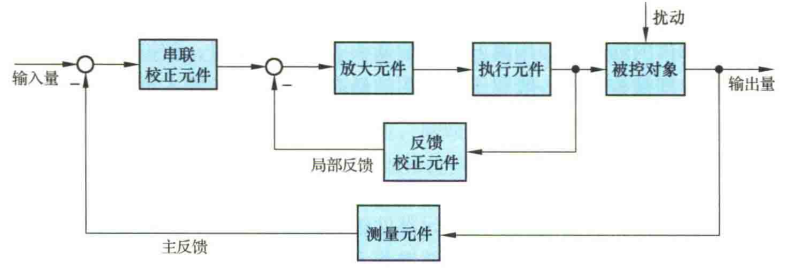
\includegraphics[width=0.8\textwidth]{feedback_diagram.png}
  \caption{反馈控制系统结构} \label{fig:feedback_diagram}
\end{figure}

如图所示,反馈控制系统的结构一目了然(当然图中还有一个局部的反馈,所以并不是一个最简单的反馈系统),串联校正元件其实就是控制器。个人有时会混淆\textbf{被制变量}和\textbf{控制变量},前者是被控对象的输出,后者是作用于控制对象的。其余的术语不多解释,随便翻开一本《自动控制原理》就能找到解答。

除了开环、闭环反馈系统,还有混合控制系统:按输入补偿的前馈、按扰动补偿的前馈结合闭环反馈系统就是了,直接上卢姥爷(卢京潮)的图。

\begin{figure}[htbp]
  \centering
  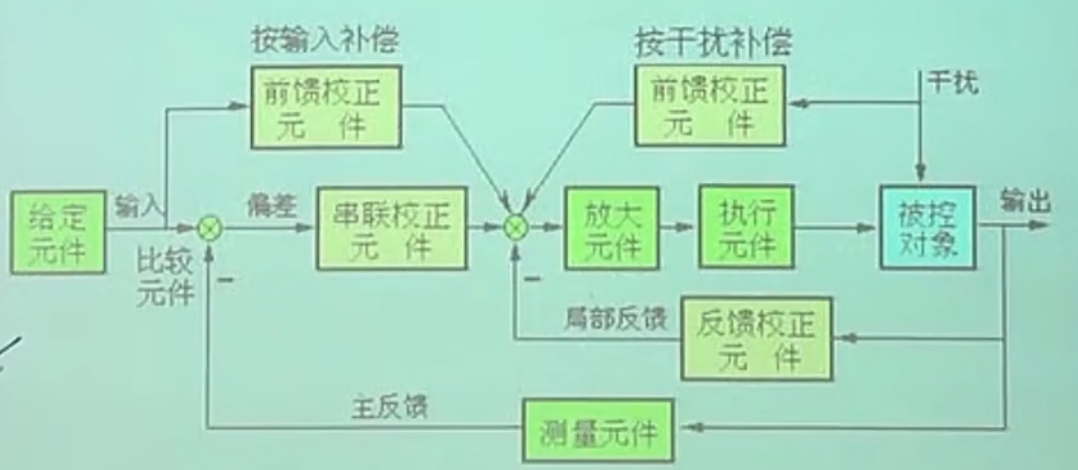
\includegraphics[width=0.8\textwidth]{hybrid_control.png}
  \caption{混合控制系统结构} \label{fig:hybrid_control}
\end{figure}

\section{控制系统分类}

控制系统的分类规则其实很简单:时变/时不变(定常),线性/非线性,连续/离散,还有很多分类方式,但重要的就这几个。\textbf{时变}是指其系数是随着时间变化的,例如$c(t)=t\cdot{r(t)}$。\textbf{线性是满足加法和数乘的},那么$c(t)=r(t)\cos\omega t+5$就不是一个线性的系统。

\section{数学基础}

\subsection{拉普拉斯变换}

为什么我们需要拉普拉斯变换呢?最主要的原因是他能将时域上的微分方程转换为复数域上的代数方程,使我们能更方便地分析一个系统。单值函数$f(t)$在$(0,\infty)$区间有定义时,$f(t)$的拉普拉斯积分
\begin{equation}
   F(s)=\int_0^{\infty} f(t)e^{-st}dt, s>0
\end{equation}
称为$f(t)$的拉普拉斯变换,记为
\[\mathscr{L}[f(t)] = F(s)\]

接下来我们介绍拉普拉斯变换的十大定理(定理和常用变换可以参考《自动控制原理题海与考研指导》):
\begin{figure}[htbp]
  \centering
  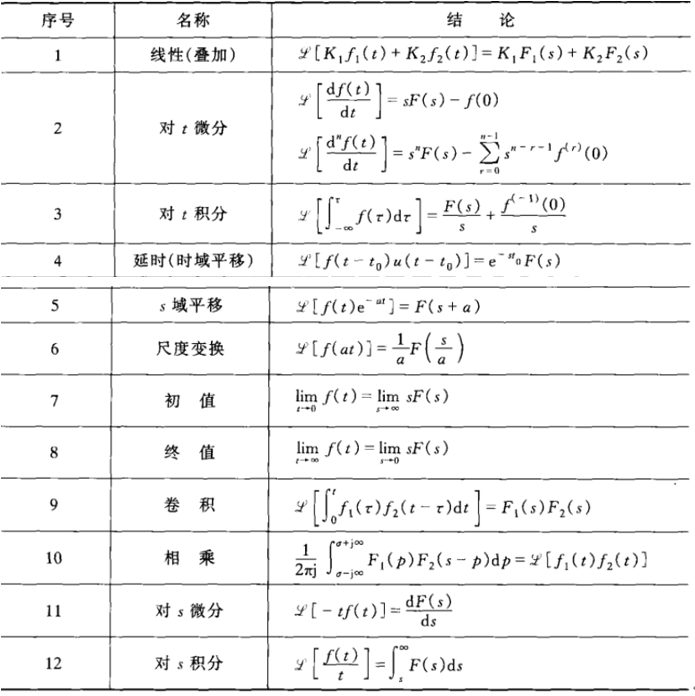
\includegraphics[width=0.8\textwidth]{l_property.png}
  \caption{拉氏变换性质表} \label{fig:l_property}
\end{figure}

注意第三项中$f^{-1}(0)=[{\int f(t) dt}]_{t=0_{\pm}}$,并且公式中没有给出高维的公式,读者可以去书上看看。

数学上,拉普拉斯反变换可以通过下述公式计算:
\begin{equation}
   f(t) = \frac{1}{2\pi j}\int_{c-j\infty}^{c+j\infty} F(s)e^{st}dt, t>0
\end{equation}
其中$c$大于所有$F(s)$奇点的实部,反变换记为:
\[f(t)={\mathscr{L}}^{-1}[F(s)]\]


计算上述公式比较麻烦,因此我们求反变换的时候常常将$F(s)$部分分式分解,然后用常见拉氏变换和留数法来做。将$F(s)$分解为如下:
\[F(s)= \frac{{b_0 s^m}+{b_1 s^{m-1}}+\dots+{b_m}}{(s-s_1)(s-s_2)\dots(s-s_n)}\]

如果没有重根,那么$F(s)=\sum\limits_{i=1}^n \frac{c_i}{s-s_i}$,其中$c_i$用留数法得到:
\begin{equation}
   c_i=\lim_{s \to s_i}(s-s_i)F(s)
\end{equation}

如果有重根,这里以$r$重根$s_1$为例,那
\[F(s)=\frac{c_r}{(s-s_1)^r} + \frac{c_{r-1}}{(s-s_1)^{r-1}}+\dots + \frac{c_1}{s-s_1}+\frac{c_{r+1}}{s-s_{r+1}}+\dots\]
其中$\displaystyle{c_{r-j}=\frac{1}{j!} \lim_{s \to s_1} \frac{d^{r-j}}{ds^{r-j}}[(s-s_1)^r F(s)]}$,然后利用常见变换即可.

\subsection{Z变换}
从拉氏变换到Z变换的过程比较简单,我们首先有信号$e(t)$,它在$t<0$时为0,我们需要对该信号采样,得到
\[e^*(t)=\sum \limits_{n=0}^{\infty}e(nT)\delta(t-nT)\]
同时注意到$\int_{0}^{+\infty} e(t)dt = \int_{-\infty}^{+\infty} e(t)dt$,那么对$e^*(t)$拉普拉斯变换就可以得到(推导过程请读者自己练习):
\[E^*(s)=\sum \limits_{n=0}^{\infty}e(nT)e^{-snT}\]
然后经过一个简单的变量代换,$s=\frac{1}{T}\ln{z}$,我们变得到了Z变换的定义(我们用$e(n)$表示$e(nT)$):
\begin{equation}
    E(z)=\mathscr{Z}[e^*(t)]=\mathscr{Z}[e(t)]=\sum \limits_{n=0}^{\infty}e(n)z^{-n}
\end{equation}

z变换的性质见:





\chapter{控制系统的数学模型}

\section{时间域建模}

这里我就讲一个线性化,$y=f(x)$,把它泰勒展开并消去高次幂则得到:
\[y-y_0=\left( \frac{\text{d}f(x)}{\text{d}x}\right)_{x_0} (x-x_0)\]
$\Delta y=y-y_0,\Delta x=x-x_0,K=(\text{d} f(x)/\text{d}x)_{x_0}$,那么去掉增量符号,我们得到$y=Kx$,我们要尤其注意到这是工作点附近展开的、近似的。

\section{复数域建模}

\begin{definition}[传递函数]
    零初始条件下,系统输出量的拉氏变换与输入量的拉氏变换之比
\end{definition}

传递函数的分子和分母经因式分解以后可以写为如下形式:
\[G(s)=\frac{b_0(s-z_1)(s-z_2)\cdots (s-z_m)}{a_0(s-p_1)(s-p_2)\cdots (s-p_n)}=K^*\frac{\prod \limits_{i=1}^m(s-z_i)}{\prod \limits_{j=1}^n(s-p_i)}\]

这就是传递函数的零极点表示法(也叫首一表示法),其中$K^*$为传递系数或\textbf{根轨迹增益},如果采用尾一表示法那$K$就称为增益或传递系数。
\[K=K^*\frac{\prod \limits_{i=1}^m(-z_i)}{\prod \limits_{j=1}^n(-p_i)} \]

\section{结构图和流图}
这里只写一个梅森增益公式:
\[P=\frac{1}{\Delta} \sum \limits_{k=1}^{n} p_k \Delta_k\]
其中$\Delta = 1-\sum L_a + \sum L_b L_c -\cdots$,$L$表示回路。在简化时注意前馈可能组成的回路,另外前向通道没有回路,负反馈回路的增益$L_a$为负。\textbf{对于一个确定的信号流图,梅森公式的特征式$\Delta$是不变的,对不同的原节点和阱节点前向通道和余因子式不同}。

对于一个闭环系统,其开环传递函数为前向通道和反馈通道增益的乘积(若为负反馈,不带负号),其实就是主反馈断开了(不与输入做加减法了)后该反馈的传递函数与输入的传递函数的比。

\section{常见元件和系统的建模}

首先是著名的基尔霍夫定律

\chapter{线性系统的时域分析法}

我们来定义几个重要的术语:
\begin{definition}[性能指标]
    \begin{enumerate}
        \item 
        \textcolor[rgb]{0.75, 0.5, 0.25}{上升时间$t_r$}为第一次到达终值的时间
        \item 
        \textcolor[rgb]{0.75, 0.5, 0.25}{峰值时间$t_p$}为到达第一个峰值的时间
        \item 
        \textcolor[rgb]{0.75, 0.5, 0.25}{调节时间$t_s$}为到达并保持在终值$\pm 5\%$的时间
        \item 
        \textcolor[rgb]{0.75, 0.5, 0.25}{超调量$\sigma$}为最大偏离值与终值的差与终值的比:
        \[\sigma \%=\frac{c(t_p)-c(\infty)}{c(\infty)} \times 100\%\]
        \item 
        \textcolor[rgb]{0.75, 0.5, 0.25}{衰减比$n$}为两次峰值与终值差的比,即$n=\sigma/B^{\prime}$
    \end{enumerate}
\end{definition}

\section{一阶系统}
一阶系统的传递函数为:
\[\phi(s)=\frac{1}{Ts+1}\]
其单位阶跃响应为$c(t)=1-e^{-t/T}$,$t_r=2.2T,t_s=3T(\Delta=5\%)$或$4T(\Delta=2\%)$。$c(T)=0.632,c(2T)=0.865,c(3T)=0.95,c(4T)=0.982$。其单位脉冲响应为$c(t)=\frac{1}{T}e^{-t/T}$,单位斜坡响应$c(t)=(t-T)+Te^{-t/T}$(稳态误差为$T$)。

一阶系统不能跟踪加速度输入函数,这里没写出单位加速度下的响应,这是因为:\textbf{系统对输入信号导数的响应,就等于系统对该输入信号响应的导数},读者对上面三个响应做下运算就可以得到检验。

\section{二阶系统}
二阶系统的传递函数为:
\[\phi(s)=\frac{k}{T_ms^2+s+K}=\frac{{\omega_n}^2}{s^2+2\zeta \omega_n +{\omega_n}^2}\]
当$0<\zeta<1,s_{1,2}=-\zeta \omega_n \pm j\omega_n \sqrt{1-{\zeta}^2}$,此时为欠阻尼情况;当$\zeta=1,s_{1,2}=-\omega_n$,此时为临界阻尼情况;当$\zeta>1,s_{1,2}=-\zeta \omega_n \pm \omega_n \sqrt{{\zeta}^2-1}$,此时为过阻尼情况;

在欠阻尼情况下得单位阶跃响应为:
\[c(t)=1-\frac{1}{\sqrt{1-{\zeta}^2}}e^{-\zeta \omega_n t} \sin{(\omega_d t+\beta)}\]
其中$\beta=\arccos{\zeta},\omega_d=\omega_n\sqrt{1-{\zeta}^2}$为阻尼震荡频率,另外记衰减系数$\sigma=\zeta \omega_n$(\textbf{注意孙的书是负的})。阻尼比$\zeta$越小,超调量越大,上升时间越短,相同阻尼比,振荡频率$\omega_n$越大响应速度越快。

接下来我们分析欠阻尼二阶系统的动态指标,$t_r=\frac{\pi-\beta}{\omega_d},~t_p=\frac{\pi}{\omega_d}, ~ \sigma \%=e^{-\pi \zeta/\sqrt{1-{\zeta}^2}}\times 100\%,~ t_s=\frac{3}{\zeta \omega_n}$(误差带为0.05时,胡的书为3.5),$t_s=\frac{4}{\zeta \omega_n}$(误差带为0.02,胡的书为4.5),$n=B/B^{\prime}=e^{2\zeta \pi/\sqrt{1-{\zeta}^2}}$。

欠阻尼系统的单位斜坡响应稳态误差为$2\zeta/\omega_n$,其实三个不同阻尼都是同样的表达式。对于两个特征值相差较大的过阻尼系统,我们可以近似为一阶系统。

\section{二阶系统性能改善}
通过增大开环增益我们可以降低阻尼,减少稳态误差,但动态性能却并不好,因此我们需要采取别的方法来进行系统性能的改善。我们直接写出PID控制的传递函数:
\[G(s)=K_c(1+T_d s+\frac{1}{T_i s})\]

采用比例-微分控制,那么可以增大阻尼,减少超调量和调节时间,且不影响常值稳态误差和自然频率。这样就允许较高的开环增益,在保证一定动态性能的条件下,减少稳态误差。当然微分作用对高噪音有放大作用,此时可以考虑测速反馈控制。

所谓的测速反馈就是传递函数为$K_t s$的负反馈线路,此时系统的开环传递函数为:
\[G(s)=\frac{\omega_n}{2\zeta+K_t \omega_n } \times \frac{1 }{s[s/(2\zeta \omega_n+K_t {\omega_n}^2 )+1] }\]
由此可以知道,测速反馈会降低系统开环增益,进而增大\textbf{斜坡输入}时的稳态误差。不过此时其阻尼变为$\zeta_d=\zeta +\frac{1}{2}K_t \omega_n$,即阻尼增大了,动态性能改善。我们可以适当增大原系统的开环增益以弥补稳态误差的损失,同时选择$K_t$使阻尼为$0.4\sim 0.8$。

\section{高阶系统}
\begin{definition}[闭环主导极点]
  在所有的闭环极点中,距离虚轴最近的极点附近没有闭环零点,而其他闭环极点远离虚轴,这个闭环极点就叫闭环主导极点,一般我们会得到一对闭环共轭主导极点  
\end{definition}

例如下面这个系统(我们先把系统化为首一的形式):
\[G(s)=\frac{8(s+2.1) }{(s+8)(s+2)(s^2+s+1)} \approx \frac{1.05}{s^2+s+1}\]

闭环零点会减少阻尼,闭环极点会增大阻你,闭环零、极点相互靠近时会互相削弱彼此对系统响应速度的影响。

\section{线性系统的稳定性分析}
稳定平衡点和不稳定平衡点(受到干扰会不会再回到原平衡点,向上凸起的土包上的车),另外还有大范围和小范围稳定的概念,这里的大小基本指的就是干扰的大小。

\begin{definition}[线性系统稳定的充要条件]
    闭环系统特征方程的所有根都在s左半平面
\end{definition}

如果有零实部的根存在,那么系统趋于常数,这时就不是渐进稳定了,于是在经典控制理论的体系中就不是稳定系统。

我们介绍劳斯判据:劳斯表的第一列全为正那么系统稳定(充要),系数改变的次数就是正实部根的数目。另外还有一个必要条件:系统特征方程的系数应该同号且都不为0。

我们使用劳斯判据会有两种特殊情况:
\begin{enumerate}
    \item 某行第一列为0,其他列都不为0或者不全为0
    \begin{enumerate}
        \item 用一个很小的正数$\epsilon$代替
        \item 原特征方程$s=1/x$,二者的正实部根个数相同
        \item 乘个$(s+1)$,不改变正实部根的数目
    \end{enumerate}
    \item 某行元素全为0(上两行成比例),此时我们要用上一行做辅助方程,该辅助方程的解就是系统的特征根,该方程的导数的系数就是对应全零行的系数
\end{enumerate}

~\par
简化的技巧:对某行同除一个正数不会改变判断结果。另外我们有时希望有个稳定的裕度$a$,那么我们令$s=z-a$代入方程得到关于z的特征方程。

\section{稳态误差计算}
当系统稳定时,我们可以计算稳态误差,它有两种定义,一般采用下一种:
\[E(s)=R(s)-C(s)H(s),~ \phi_e(s)=\frac{1}{1+G(s)H(s)}\]

通过终值定理计算误差是要注意:$sE(s)$的极点均在s左半平面(包括坐标原点)。当有干扰时,误差是两项的和,将新的$C(s)$代入上面左边的公式即可。

举个不解析的例子:
\[E(s)=\frac{\omega s}{(s+1/T)(s^2+\omega^2)}\]
因为有虚轴上的不解析点,所以用终值定理得到稳态误差为0的结论是错的。

一般情况下,开环传递函数可以表示为(尾一标准型):
\[G(s)H(s)=\frac{K\prod\limits_{i=1}^m (\tau_i s+1)}{s^v \prod\limits_{j=1}^{n-v}(T_j s +1)}\]
其中$v$就是系统的型,那么系统的稳态误差就是:
\[e_{ss}(\infty)=\frac{\lim\limits_{s \to 0}[s^{v+1}R(s)]}{K+\lim\limits_{s \to 0}s^v}\]

稳态误差系数越大,相应的稳态误差就越小。另外注意加速度输入是指$r(t)=Rt^2/2$,当系统输入是$r(t)=R_0 \times 1(t)+R_1t+R_2t^2/2$时,我们的稳态误差可由线性叠加得到:
\[e_{ss}(\infty)=\frac{R_0}{1+K_p}+\frac{R_1}{K_v}+\frac{R_2}{K_a}\]

\begin{figure}[htbp]
  \centering
  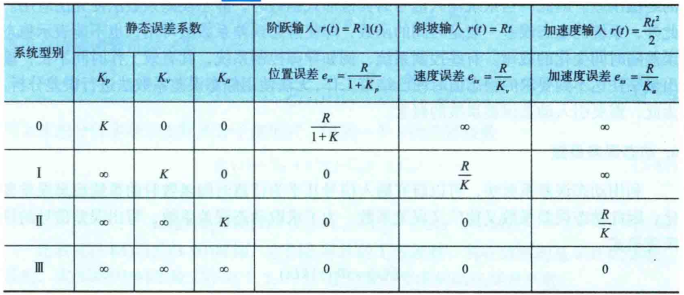
\includegraphics[width=0.8\textwidth]{k_pva.png}
  \caption{输入信号下的稳态误差} \label{fig:k_pva}
\end{figure}

减少稳态误差的措施:
增大开环增益或扰动点之前的前向通道增益;前向通道或主反馈通道设置串联积分环节(增大系统的型);而当系统有多个扰动信号时,宜采用串级控制方式。除此以外,当然还有复合控制方法。
\chapter{根轨迹分析法}

\section{基本概念}

将前向通道和反馈通道都写为首一的形式,那么我们可以得到闭环传递函数:
\[\phi(s)=\frac{K_G^* \prod\limits_{i=1}^f (s-z_i) \prod\limits_{j=1}^
h (s-p_j)}{\prod\limits_{i=1}^
n (s-p_i) + K^* \prod\limits_{j=1}^m (s-z_j)} \]
其中$f,h,m,n$分别是反馈和前向的零极点数,闭环系统根轨迹增益等于前向通道根轨迹增益,对于单位反馈闭环零点就是开环零点。

当系统的开环零点和极点有$m,n$个时我们可以得到相角条件(绘制根轨迹的充要条件):
\[\sum\limits_{j=1}^m \angle(s-z_j)-\sum\limits_{i=1}^n\angle(s-p_j)=(2k+1)\pi\]
$k=0,\pm1,\pm2,\cdots$,另外还有模值条件:
\[K^*=\frac{\prod\limits_{i=1}^n|s-p_i|}{\prod\limits_{j=1}^m|s-z_j|}\]

\section{基本法则}

\begin{figure}[htbp]
  \centering
  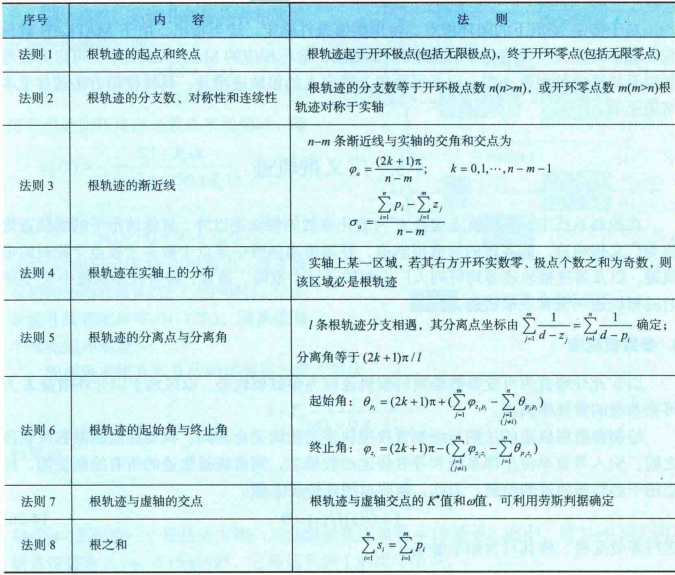
\includegraphics[width=0.8\textwidth,height=0.65\textwidth]{root_diagram_law.png}
  \caption{输入信号下的稳态误差} \label{fig:root_diagram_law}
\end{figure}

一些技巧点:
\begin{enumerate}
    \item 如果实轴上两个极点(零点同理,注意无穷极点、零点也同样)中间存在根轨迹,那至少有一个分离点。
    \item 如果两个极点一个有限零点,且零点不在两个极点中间(复数极点当然就不在中间了),那必然存在一圆以零点为圆心,零点到分离点为半径。
    \item 如果没有零点,那么$\sum_{i=1}^{n} \frac{1}{d-p_i}=0$.
    \item $n-m=1$时不必计算渐近线。
    \item 如果零点(有限或无限)和极点间有根轨迹,那么要么没有分离点,要么有两个分离点,一个离开实轴,一个进入实轴。
    \item \textbf{注意根之和是闭环的极点和开环的极点}
\end{enumerate}

~\par
\textcolor[rgb]{0.75, 0.5, 0.25}{如何通过阻尼比知道系统的闭环主导极点},我们以下面这个系统为例:
\[G(s)=\frac{K}{s(s+1)(s+5)}\]
其中$\zeta=0.45$,在图上我们去一条$\cos{\beta}=0.45$的射线与根轨迹的交点就是闭环主导极点,那么我们可以设闭环主导极点为$\sigma \pm \tan{\beta} \times \sigma i$,通过上文6我们可以得到:
\[-2\sigma +s_i = -1-5\]
即$s_i = 2\sigma-6$,得到闭环特征方程$(s-\sigma-\tan{\beta} \times \sigma)(s-\sigma+\tan{\beta} \times \sigma)(s-s_i)$,它等于$s(s+1)(s+5)+K$,对比两式就可以得到根和增益了。

\section{广义根轨迹}
对于参数的根轨迹,此处我们引入等效传递函数的概念,将闭环特征方程改写为:
\[A\frac{P(s)}{Q(s)}=-1\]
其中$P(s),Q(s)$都是跟$A$无关的,于是我们可以按照上文方法对该参数做根轨迹。

我们说等效,这只是闭环极点相同,闭环零点是不同的,我们在分析\textbf{动态性能}的时候要考虑原来闭环系统的零点。附加开环零点有助于改善稳定性,但动态性能要综合考虑。

\begin{definition}[非最小相位系统]
    系统存在位于右半平面的开环零极点,那这个系统就叫非最小相位系统
\end{definition}

对于非最小相位系统,我们的相位条件改了,所以有三个规则要更改:
\begin{enumerate}
    \item 渐近线的夹角的分子改为$2k\pi$.
    \item 实轴上若右方开环实数零极点的和为偶数(零也是偶数),那必是根轨迹。
    \item 起始角和终止角也是%2k\pi$.
\end{enumerate}

\section{基于根轨迹的补偿方式}
为了改善系统的动态性能,我们可以采用PD补偿器:$G_c = K_ds+1$,这样理论上我们改善了,但是实际上这样的系统我们无法制造,而且还增大了高频噪音,因此我们还需要配置一个极点,即:
\[G_c = A \frac{s+\frac{1}{T}}{s+\frac{1}{\alpha T}}\]
此处的$\alpha$一般选择为0.1,这样的补偿器我们称之为超前补偿器,因为其零点比极点更靠近虚轴,产生的相位为正。

当我们用超前补偿器获得不错的动态性能后,我们可能还得解决稳态误差的问题,因此我们引入滞后补偿器(类PI控制),其传递函数同上,只是$\alpha$为大于1的值,一般取10.

另外我们还可以用\textbf{极点配置法}来设计PID控制器,通过需要的参数我们得到主导极点,再选择剩下的极点(例如主导极点实部的5倍),通过特征方程比对来设计PID控制器的三个参数$K,T_i,T_d$,这种方式跟我上文讲的通过阻尼比得到闭环主导极点的方法有异曲同工之妙。

\section{习题}
\begin{exercise}
    开环传递函数为的单位负反馈系统:
    \[G(s) = \frac{K_1}{s^2+(2+K_1K_2)s+K_1}\]
    要求:用根轨迹法,斜坡输入下稳态误差小于斜坡输入常数的0.35;主导极点的阻尼比大于0.707;阶跃响应的调节时间小于3s($\Delta=2\%$)。(答案详见胡P189/680)
\end{exercise}



\chapter{频率特性分析法}

\section{概述}
对于一个线性系统,我们输入一个正弦信号,得到的也是正弦输出,例如输入$x(t) = A\sin{(\omega t + \phi)}$,得到的是:
\[y_s(t) = A|G(j\omega)|\sin(\omega t + \phi +\psi)\]
其中$\psi(\omega)=\angle G(j\omega)$,然后我们就可以对$G(j\omega)$画图了,重点是幅相曲线和BODE图,典型环节的幅相曲线和BODE图请直接参考孙优贤老师的书,还是比较清楚的!

\begin{figure}[htbp]
  \centering
  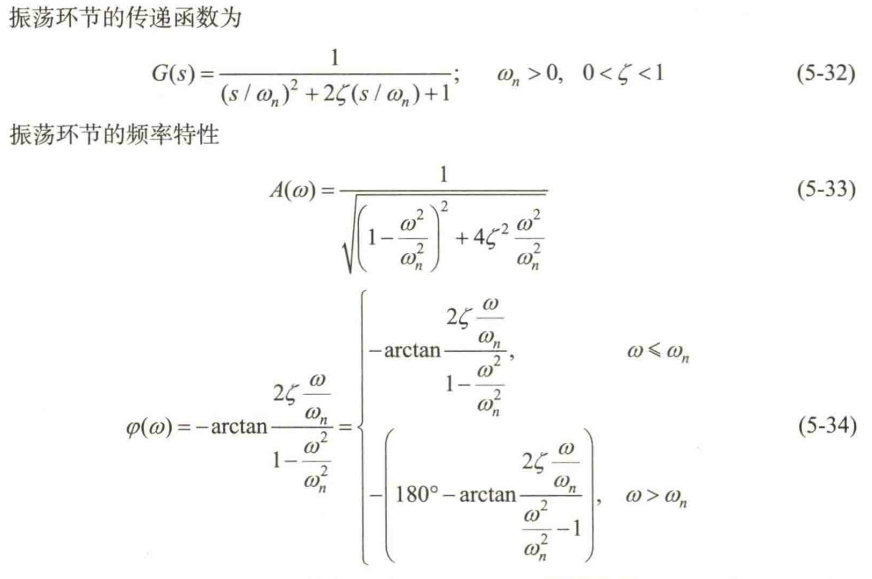
\includegraphics[width=0.8\textwidth]{image/phase_two.png}
  \caption{震荡环节的相位} \label{fig:phase_two}
\end{figure}

\textcolor[rgb]{0.75, 0.5, 0.25}{胡书上关于奈奎斯特绕圈的内容比孙的多,而且采用的是正、负穿越的说法,竟然还有半次穿越!}



\section{基于频域的补偿器设计}
还是孙老师的书,非常清楚明了了!

\chapter{线性控制系统的校正方法}

\chapter{线性离散系统的分析与校正}

\chapter{非线性系统分析}

\chapter{线性系统的状态空间分析与综合}

\chapter{最优控制方法}

这部分要考吗?

\end{document}